% Commande pour générer le document au format pdf
% latex-mk --pdflatex myschool.tex

% TODO
% Structure de la base de données Sqlite

\documentclass{article}
\usepackage{graphicx}
\usepackage{titlesec}
\usepackage{fullpage}
\usepackage{pdflscape}
\usepackage{adjustbox}
\usepackage[table]{xcolor}    % utilisation de "rowcolor"
\usepackage[
   colorlinks=true,
   linkcolor=blue,
   citecolor=blue]{hyperref}
\usepackage{hyperref}         % liens hypertexte dans la table des matières
\usepackage{makecell}

\title{\parbox{10cm}{
   \begin{center}\sf\bfseries\huge
      \hrule
      
\includegraphics[width=8cm]{images/myschool.png} \\
      \hrule
   \end{center}
   \hfill\scriptsize Arnaud ETCHEVERRY  - 1 juin 2026\\[2cm]
}}
\author{}
\date{}

\begin{document}

\maketitle

% Table des mises à jour
\textbf{MISES A JOUR} \\
\\
\begin{adjustbox}{width=1.2\textwidth,center}
\resizebox{\textwidth}{!}{
\begin{tabular}{|p{2cm}|p{2cm}|p{6cm}|p{8cm}|}
   \hline
   \rowcolor{gray!30}
   \textbf{Version} & \textbf{Date} & \textbf{Auteur} & \textbf{Modifications} \\
   \hline
   \textbf{1.0} & 01/06/2026 & Arnaud ETCHEVERRY & Version initiale \\
   \hline
\end{tabular}
}
\end{adjustbox}

% Table des References
\newpage
\textbf{REFERENCES} \\
\\
\begin{adjustbox}{width=1.2\textwidth,center}
\begin{small}
\begin{tabular}{|p{1.5cm}|p{14cm}|}
   \hline
   \rowcolor{gray!30}
   \textbf{REF} & \textbf{Titre} \\
   \hline
   \textbf{REF\_1} & \makecell[l]{\textbf{Howto - Tree view} \\ \href{https://www.w3schools.com/HOWTO/howto\_js\_treeview.asp/}{\textcolor{blue}{https://www.w3schools.com/HOWTO/howto\_js\_treeview.asp}}} \\
   \hline
   \textbf{REF\_2} & \makecell[l]{\textbf{Managing trees in Mysql using the Adjacency List Model} \\ \href{https://rolandgeng.de/managing-trees-in-mysql-using-the-adjacency-list-model}{\textcolor{blue}{https://rolandgeng.de/managing-trees-in-mysql-using-the-adjacency-list-model}}} \\
   \hline
   \textbf{REF\_3} & \makecell[l]{\textbf{Sqlite foreign key support} \\ \href{https://www.sqlite.org/foreignkeys.html}{\textcolor{blue}{https://www.sqlite.org/foreignkeys.html}}} \\
   \hline
   \textbf{REF\_4} & \makecell[l]{\textbf{Trees hierarchies in SQL for smarties} \\ \href{}{\textcolor{blue}{}}} \\
   \hline
   \textbf{REF\_5} & \makecell[l]{\textbf{Database normalization} \\ \href{https://en.wikipedia.org/wiki/Database\_normalization}{\textcolor{blue}{https://en.wikipedia.org/wiki/Database\_normalization}}} \\
   \hline
   \textbf{REF\_6} & \makecell[l]{\textbf{Custom context menu} \\ \href{https://www.youtube.com/watch?v=-R8\_MswrzD8}{\textcolor{blue}{https://www.youtube.com/watch?v=-R8\_MswrzD8}}} \\
   \hline
   \textbf{REF\_7} & \makecell[l]{\textbf{Managing hierarchical data in Mysql using the Adjacency List Model} \\ \href{https://www.mysqltutorial.org/mysql-adjacency-list-tree}{\textcolor{blue}{https://www.mysqltutorial.org/mysql-adjacency-list-tree}}} \\
   \hline
   \textbf{REF\_8} & \makecell[l]{\textbf{Apache : The definitive guide - third edition}} \\
   \hline
   \textbf{REF\_9} & \makecell[l]{\textbf{CSS : The definitive guide - fifth edition}} \\
   \hline
\end{tabular}
\end{small}
\end{adjustbox}

\newpage
\tableofcontents

% Introduction
\newpage
\section{Introduction}
 \textbf{MySchool} est une application qui permet de construire sa propre base de données de raccourcis Internet. \\
Elle offre la possibilité d'ajouter, de modifier ou de supprimer une liste de raccourcis Internet. \\
Il s'agit d'une application multi utilisateurs dans le sens ou chaque entrée dans la base de données est associée à un utilisateur.
\begin{center}
\includegraphics[width=18cm,keepaspectratio]{images/myschool\_homepage.png}
\end{center}

% Architecture logicielle
\newpage
\section{Architecture logicielle}
\vspace{2em}
\begin{center}
\includegraphics[width=18cm,keepaspectratio]{images/myschool\_software\_architecture.png}
\end{center}
\vspace{2em}
L'application \textbf{MySchool} est avant tout une application basée autour d'une base de données Sqlite.
L'exploitation de cette base de données s'effectue à travers les étapes suivantes :
\begin{enumerate}
   \item La page d'accueil de l'application correspond à une page d'authentification
      \begin{center}
      \includegraphics[width=6cm,keepaspectratio]{images/connexion\_page.png}
      \end{center}
   \item Si on entre un login et un password l'application nous redirige vers la page \textbf{connexion.php} lorsqu'on clique sur le bouton \textbf{Connexion}. \\
   Si on appuie sur le bouton \textbf{Inscription} on est dirigé vers la page \textbf{inscription.php}
   \item Aprés validation des identifiants on est dirigé vers la page \textbf{myschool.php}
      \begin{center}
      \includegraphics[width=18cm,keepaspectratio]{images/myschool\_homepage.png}
      \end{center}
   Cette page va interroger la base de données pour extraire tous les items correspondant à l'utilsateur.
   Cette extraction conduit à la construction du fichier \textbf{myschool.xml}
   \item Pour afficher les items de manière arborescente on va utiliser l'outil \textbf{xsltproc} qui va convertir la page myschool.xml en \textbf{myschool.html} \\
   Le fichier \textbf{myschool.xsl} décrit la manière dont va être conduite cette transformation.
      \newpage
      \begin{center}
      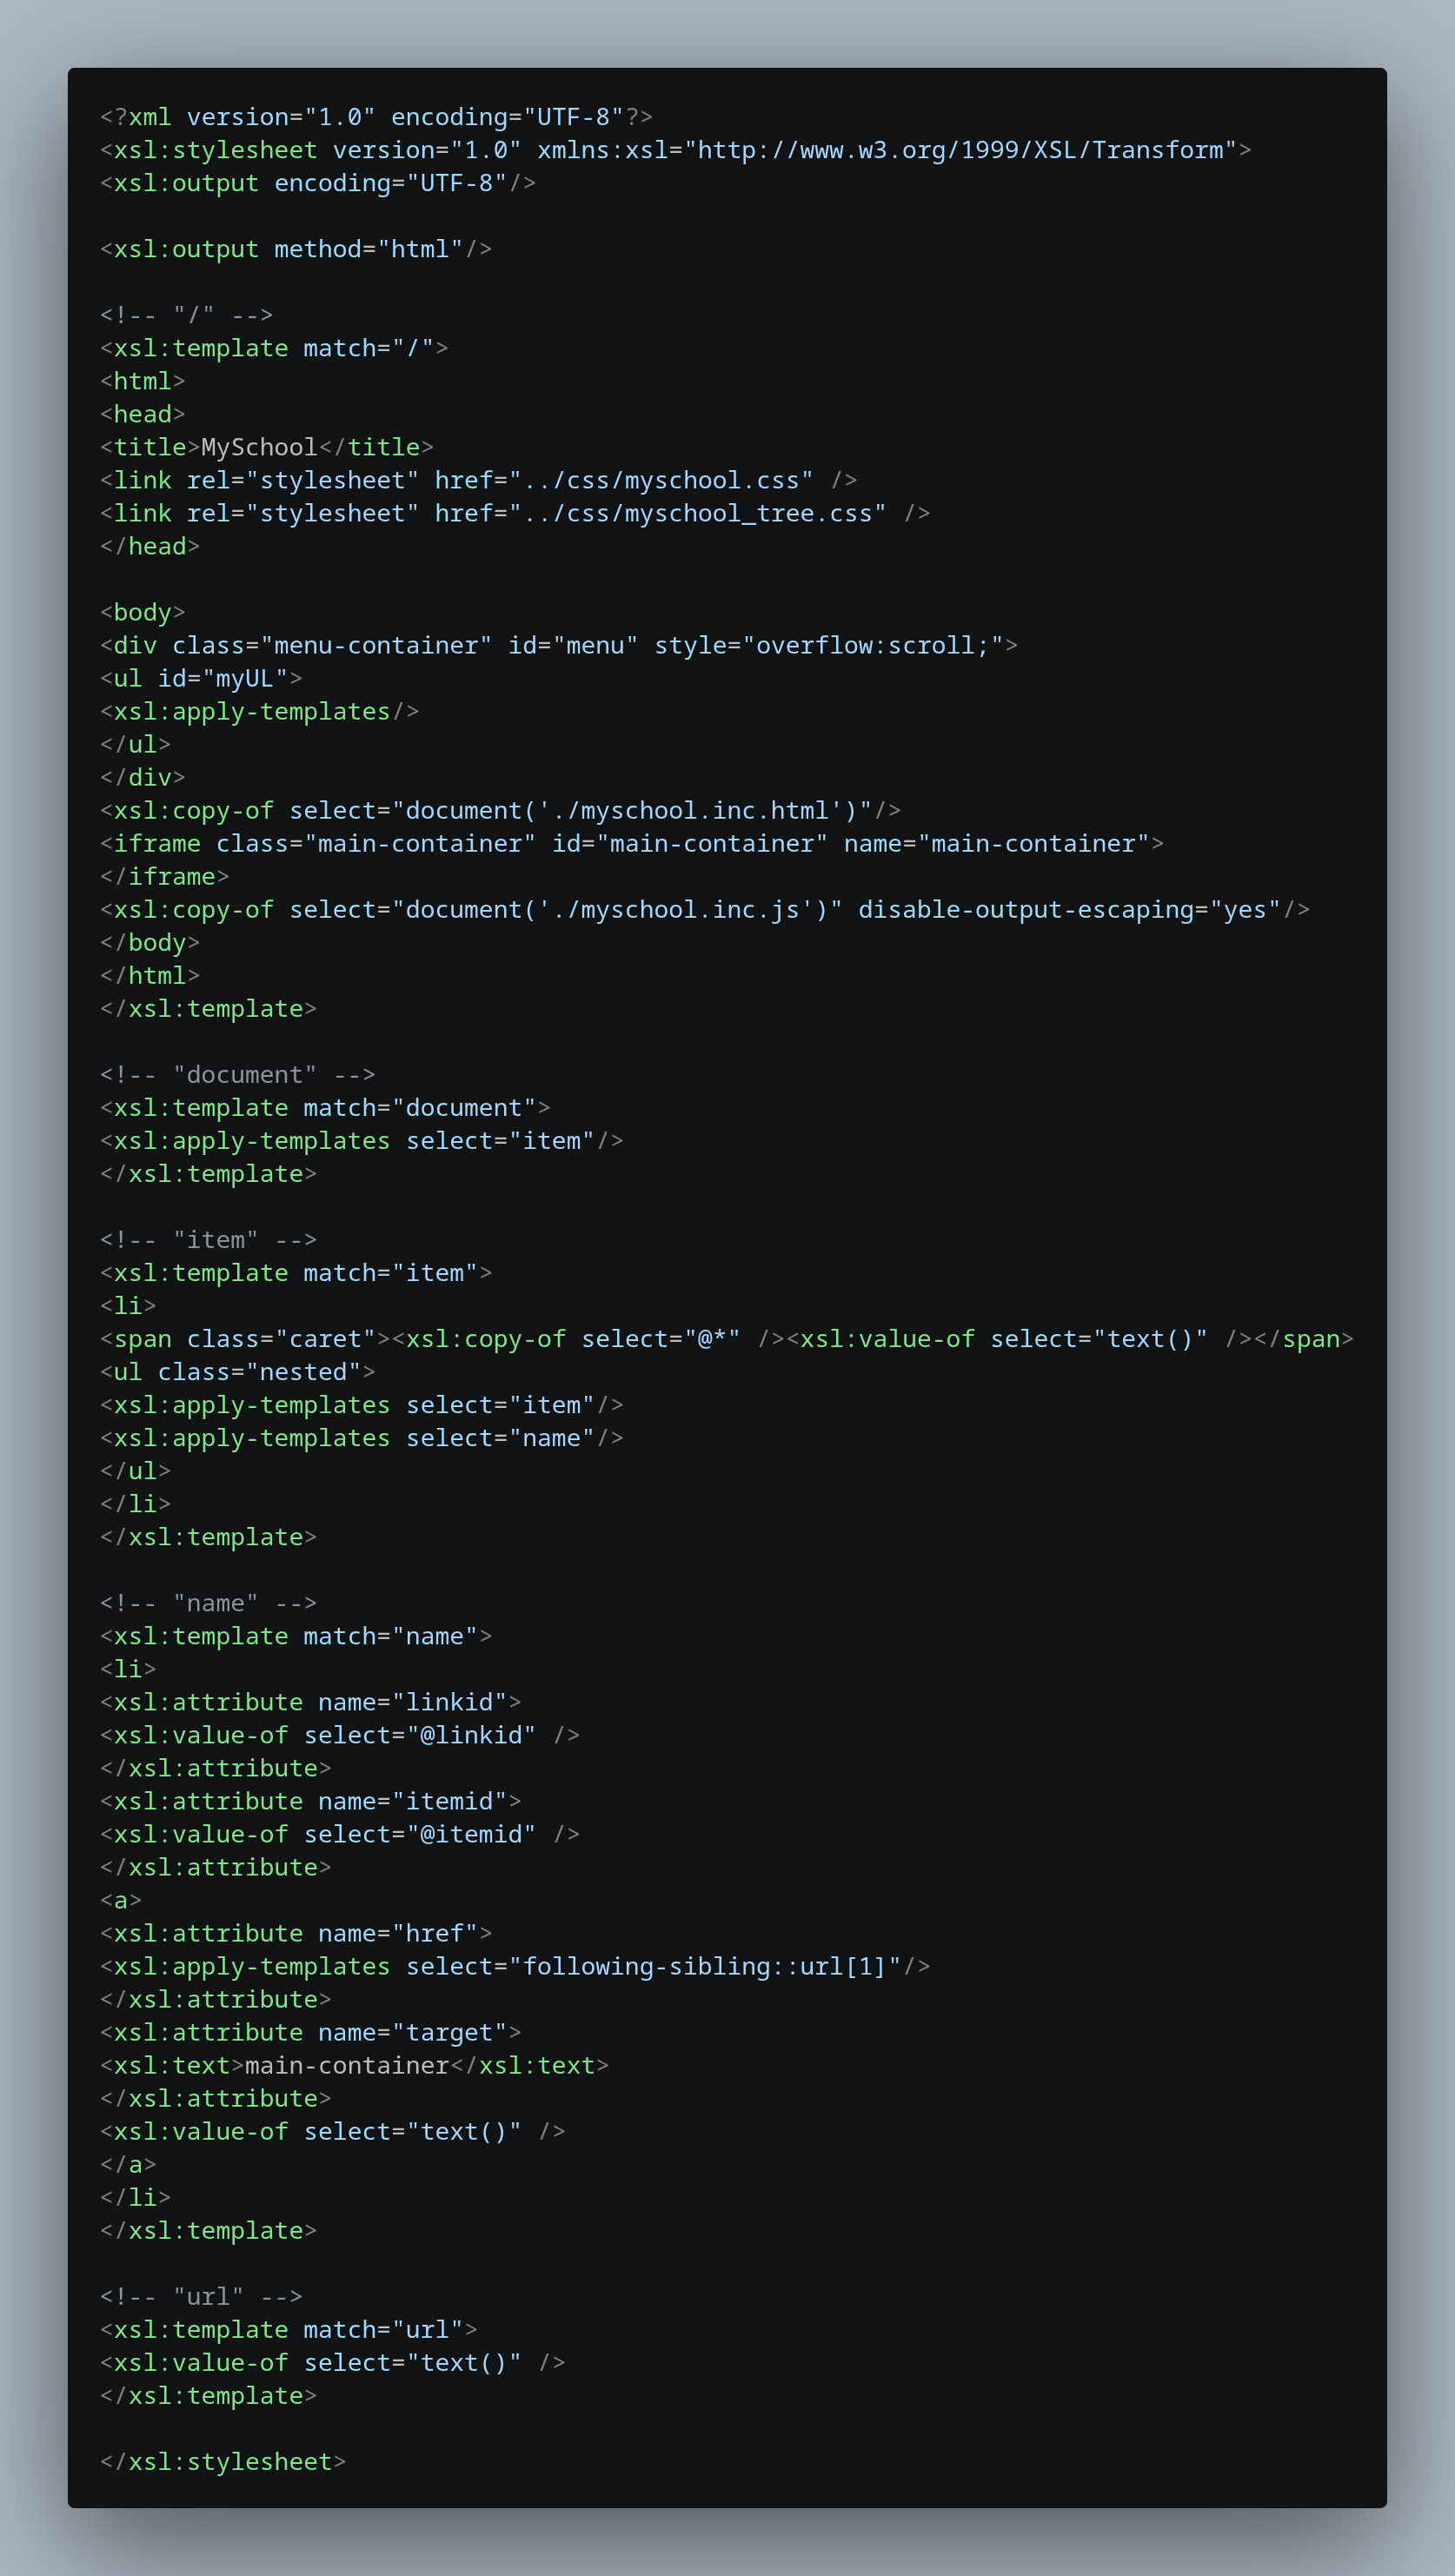
\includegraphics[width=14cm,keepaspectratio]{images/myschool.xsl.png}
      \end{center}
\end{enumerate}

% Connexion au site Myschool
\newpage
\section{Connexion au site Myschool}
\vspace{2em}
\begin{center}
\includegraphics[width=18cm,keepaspectratio]{images/myschool\_connexion.png}
\end{center}
\vspace{2em}
\begin{center}
\includegraphics[width=6cm,keepaspectratio]{images/connexion\_page.png}
\end{center}

% Gestion d'une liste arborescente
\newpage
\section{Gestion d'une liste arborescente}
\resizebox{\textwidth}{!}{
\begin{tabular}{|p{1.5cm}|p{12.5cm}|}
   \hline
   \rowcolor{gray!30}
   \textbf{REF} & \textbf{Titre} \\
   \hline
   \textbf{REF\_2} & \makecell[l]{\textbf{Managing trees in Mysql using the Adjacency List Model} \\ \href{https://rolandgeng.de/managing-trees-in-mysql-using-the-adjacency-list-model}{\textcolor{blue}{https://rolandgeng.de/managing-trees-in-mysql-using-the-adjacency-list-model}}} \\
   \hline
\end{tabular}
}

% Gestion des items en XML
\newpage
\section{Gestion des items en XML}

% Conversion du fichier XML en HTML
\newpage
\section{Conversion du fichier XML en HTML}

% Gestion des données en base de données Sqlite
\newpage
\section{Gestion des données en base de données Sqlite}
\resizebox{\textwidth}{!}{
\begin{tabular}{|p{1.5cm}|p{12.5cm}|}
   \hline
   \rowcolor{gray!30}
   \textbf{REF} & \textbf{Titre} \\
   \hline
   \textbf{REF\_2} & \makecell[l]{\textbf{Managing trees in Mysql using the Adjacency List Model} \\ \href{https://rolandgeng.de/managing-trees-in-mysql-using-the-adjacency-list-model}{\textcolor{blue}{https://rolandgeng.de/managing-trees-in-mysql-using-the-adjacency-list-model}}} \\
   \hline
\end{tabular}
}
\\
\\
\\
\resizebox{\textwidth}{!}{
\begin{tabular}{|p{1.5cm}|p{12.5cm}|}
   \hline
   \rowcolor{gray!30}
   \textbf{REF} & \textbf{Titre} \\
   \hline
   \textbf{REF\_3} & \makecell[l]{\textbf{Sqlite foreign key support} \\ \href{https://www.sqlite.org/foreignkeys.html}{\textcolor{blue}{https://www.sqlite.org/foreignkeys.html}}} \\
   \hline
\end{tabular}
}
\\
\\
\\
\begin{center}
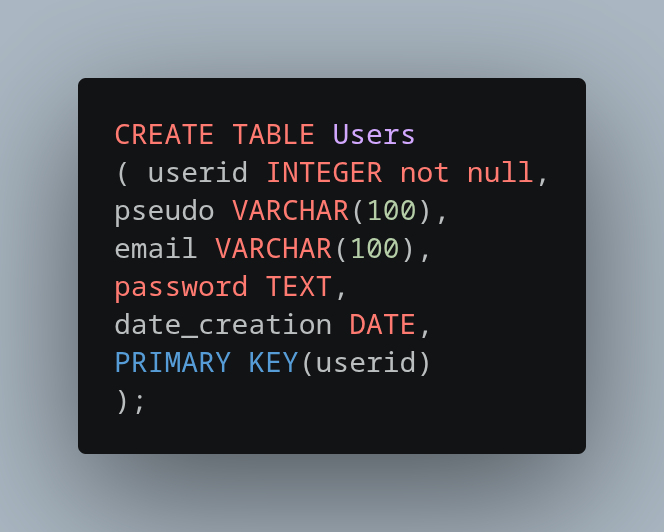
\includegraphics[width=7cm,keepaspectratio]{images/sqlite_table_users.png}
\end{center}
\begin{center}
\begin{adjustbox}{width=1.2\textwidth,center}
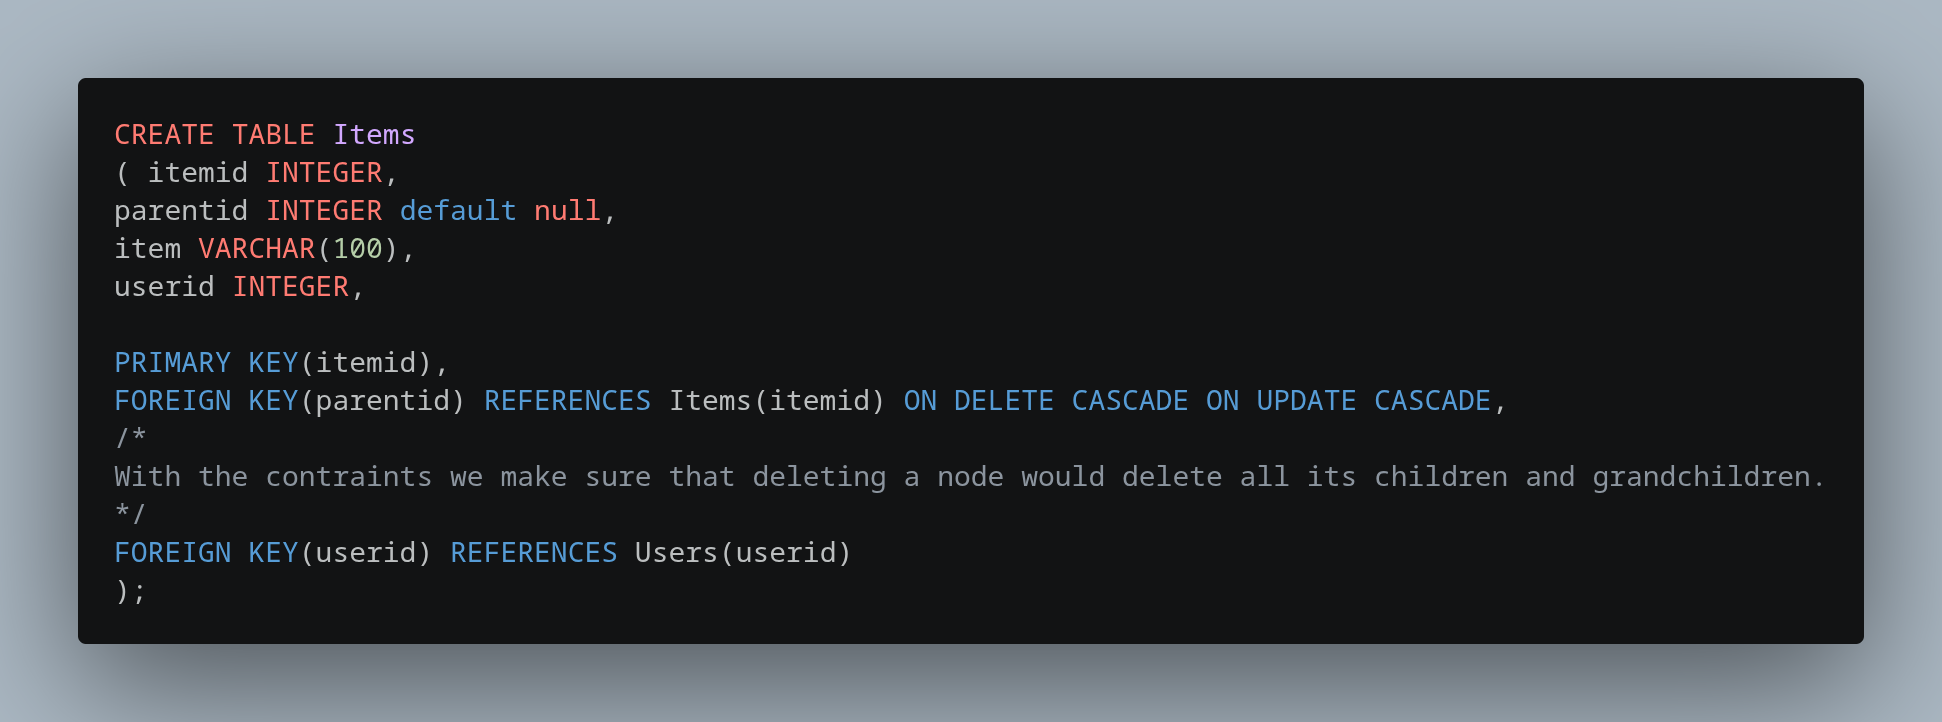
\includegraphics[width=20cm,keepaspectratio]{images/sqlite_table_items.png}
\end{adjustbox}
\end{center}
\begin{center}
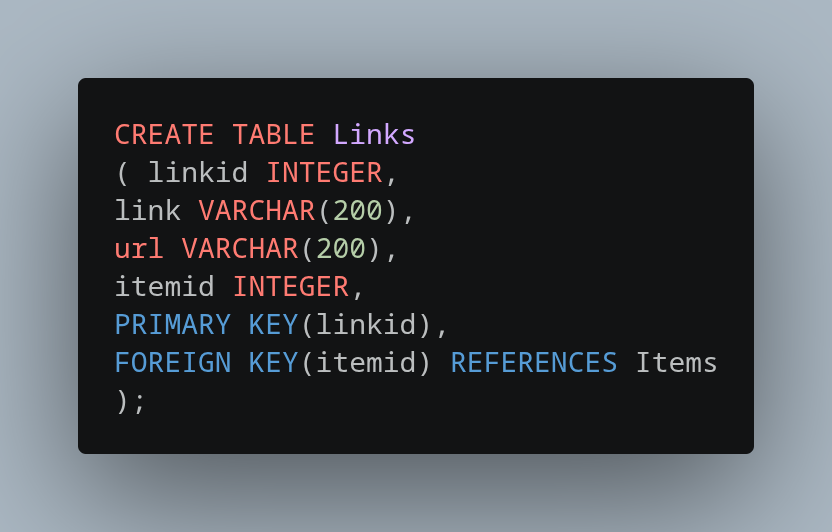
\includegraphics[width=10cm,keepaspectratio]{images/sqlite_table_links.png}
\end{center}

% Gestion du menu contextuel
\newpage
\section{Gestion du menu contextuel}
\resizebox{\textwidth}{!}{
\begin{tabular}{|p{1.5cm}|p{12.5cm}|}
   \hline
   \rowcolor{gray!30}
   \textbf{REF} & \textbf{Titre} \\
   \hline
   \textbf{REF\_6} & \makecell[l]{\textbf{Custom context menu} \\ \href{https://www.youtube.com/watch?v=-R8\_MswrzD8}{\textcolor{blue}{https://www.youtube.com/watch?v=-R8\_MswrzD8}}} \\
   \hline
\end{tabular}
}

% Gestion du serveur Apache
\newpage
\section{Gestion du serveur Apache}
\begin{center}
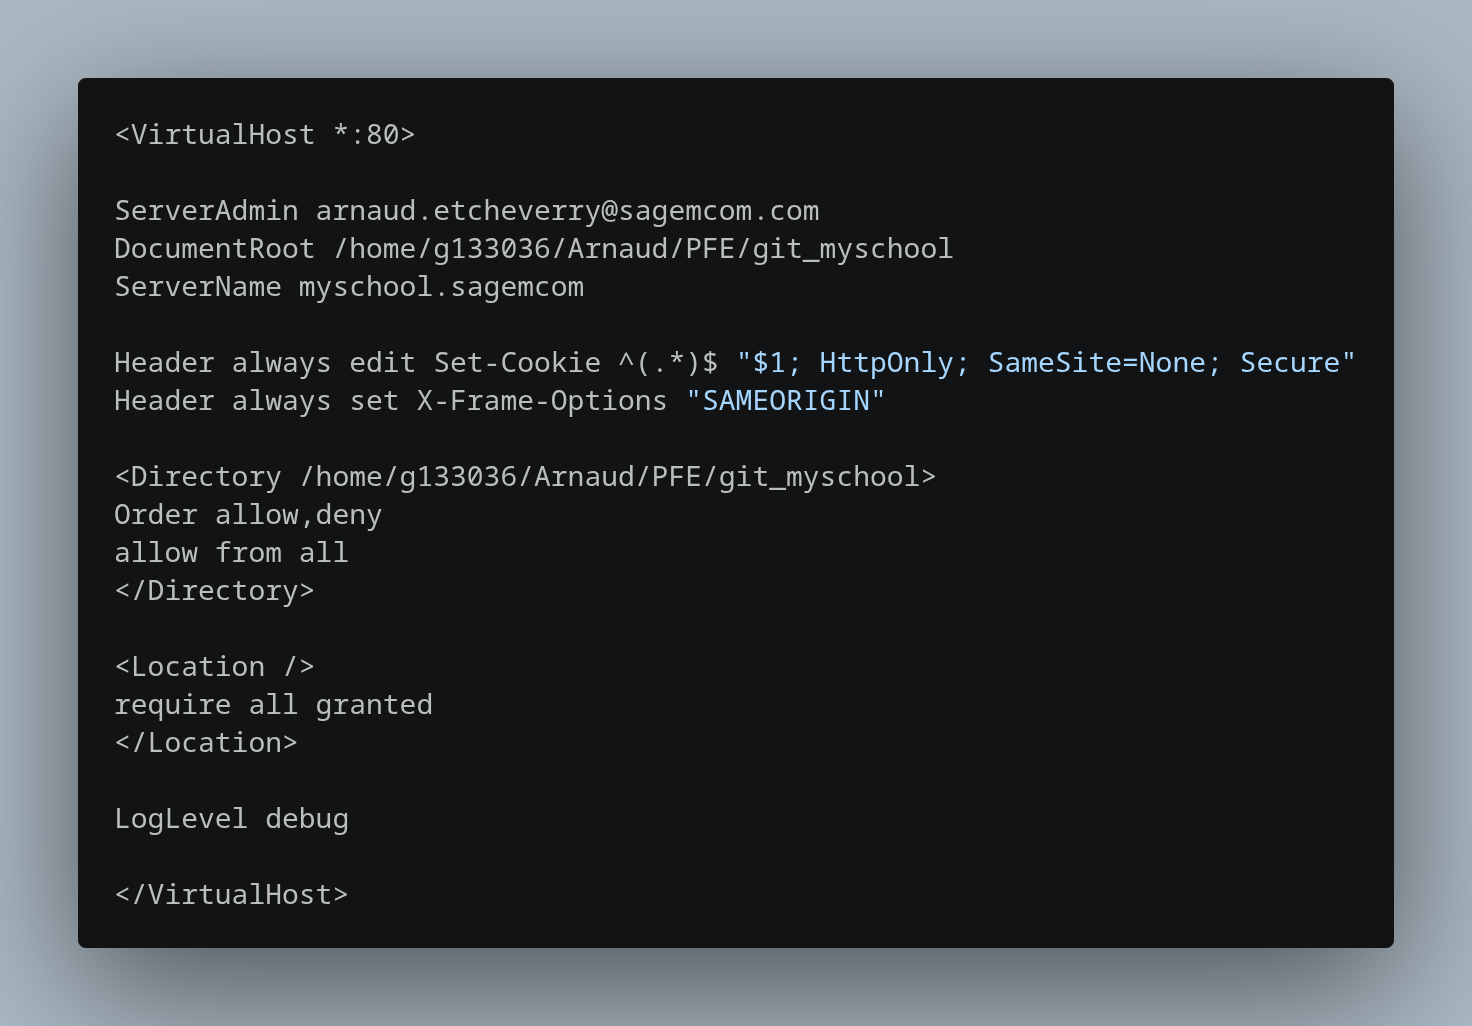
\includegraphics[width=15cm,keepaspectratio]{images/myschool.conf.png}
\end{center}

% Prise en charge du PHP
\newpage
\section{Prise en charge du PHP}

% Prise en charge de SQLite
\newpage
\section{Prise en charge de SQLite}

% Gestion des utilisateurs
\newpage
\section{Gestion des utilisateurs}

% Outils
\newpage
\section{Outils}

% Création du fichier XML depuis la base de données SQLite
\subsection{Création du fichier XML depuis la base de données SQLite}
\begin{center}
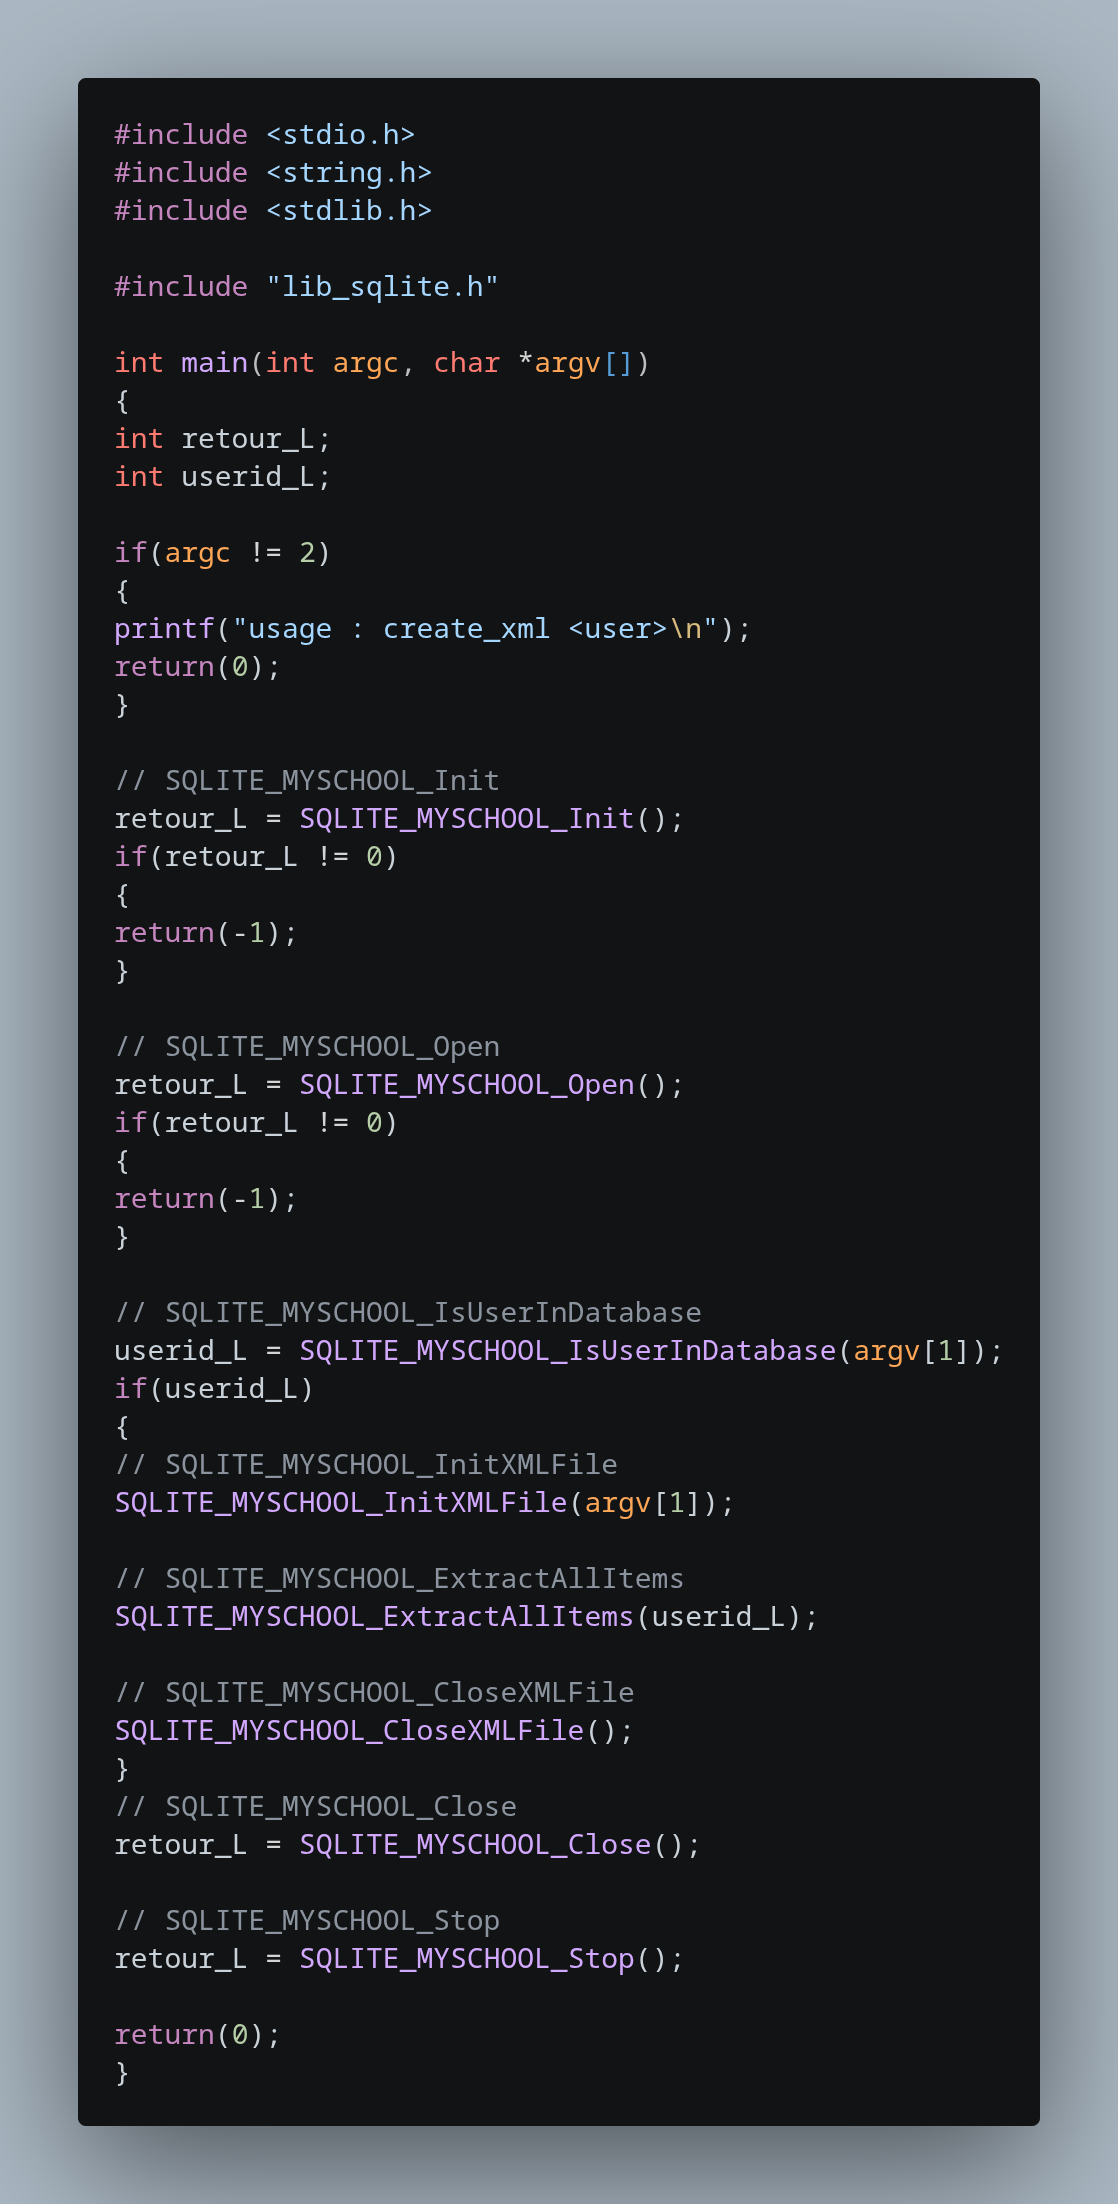
\includegraphics[width=10cm,keepaspectratio]{images/create_xml.c.png}
\end{center}

% Création de la base de données SQLite à partir d'un fichier XML
\subsection{Création de la base de données SQLite à partir d'un fichier XML}
\begin{center}
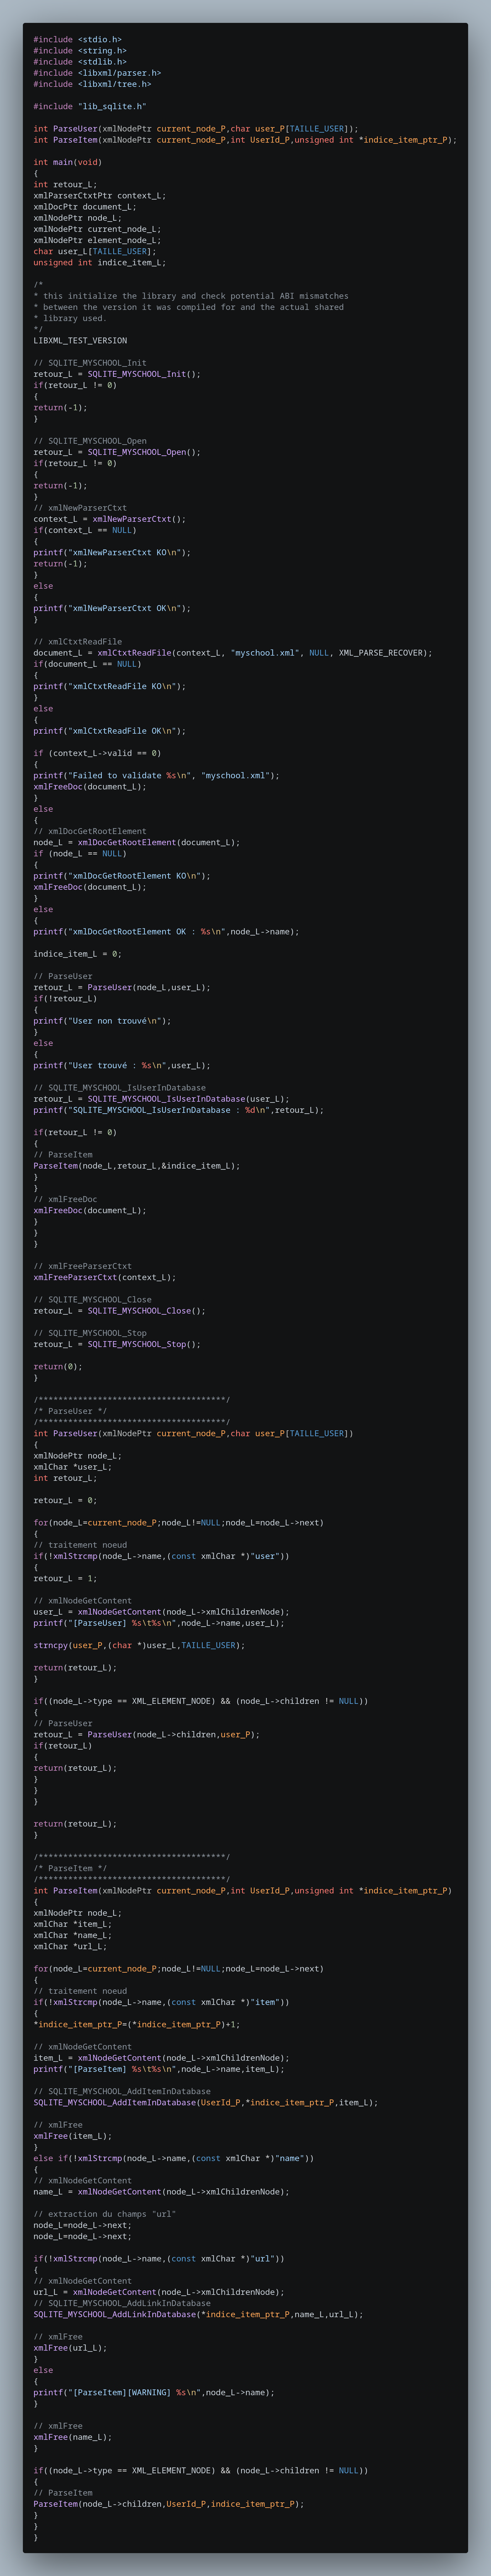
\includegraphics[width=13cm,keepaspectratio]{images/create_database.c.png}
\end{center}

% Plan de tests
\newpage
\section{Plan de tests}

% Annexe 1 : Installation du serveur Apache
\newpage
\section{Annexe 1 : Installation du serveur Apache}

\end{document}
